\documentclass{standalone}
\usepackage{preset}
\begin{document}
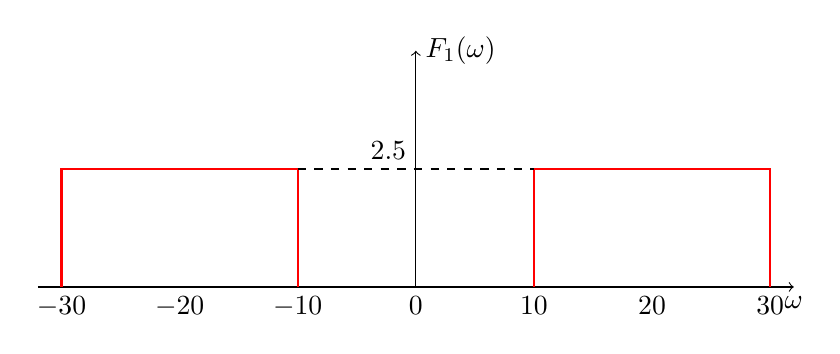
\begin{tikzpicture}[x=15mm,y=15mm]
    \draw[->](-3.2,0)--(3.2,0)node[below]{\(\omega\)};
    \draw[->](0,0)--(0,2)node[right]{\(\abs{F_1(\omega)}\)};
    \foreach \x/\label in {-3/$-30$,-2/$-20$,-1/$-10$,0/$0$,1/$10$,2/$20$,3/$30$}{
        \draw(\x,0)node[below]{\label};
    }
    \draw(0,1)node[above left]{$2.5$};
    \draw[red,thick](-3,0)--(-3,1)--(-1,1)--(-1,0);
    \draw[red,thick](3,0)--(3,1)--(1,1)--(1,0);
    \draw[dashed,thick](-1,1)--(1,1);
\end{tikzpicture}
\end{document}
